\newpage
\section{Durchführung}
\label{sec:Durchfuehrung}
\subsection{Aufbau}
    \begin{figure}[h]
        \center
        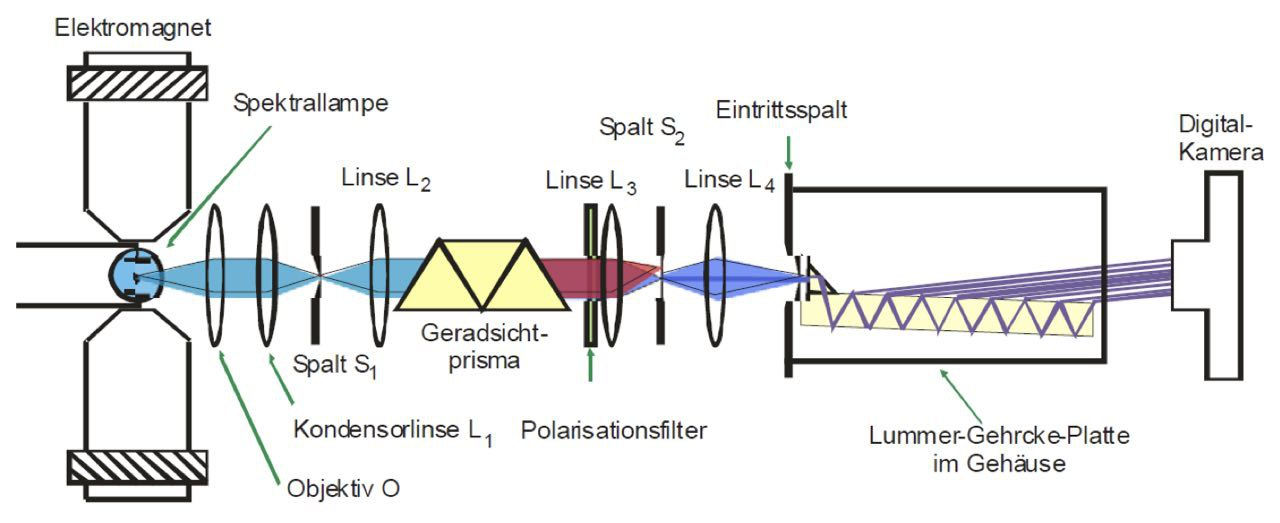
\includegraphics[width=0.7\textwidth]{bilder/aufbau.jpeg}
        \caption{Der schematische Aufbau des Versuchs ist hier dargestellt. \cite{tu_dortmund_versuchsanleitung_2021}}
        \label{fig:aufbau}
    \end{figure}
    \FloatBarrier

    Eine Cadmium-Spektrallampe wird zwischen die Pole eines Elektromagneten gestellt.
    Das Licht senkrecht zum Magnetfeld soll im weiter Verlauf des Versuches betrachtet werden, weshalb der Strahlengang auch senkrecht zum Magnetfeld aufgebaut ist.
    Das ausgesandte Licht wird am Objektiv O kollimiert und danach durch die Kondensatorlinse L$_1$ auf den Spalt S$_1$ fokussiert.
    Weiterhin wird das Licht durch die Linse L$_2$ kollimiert und durch das Geradsichtprisma gesandt, welches das Licht, aufgrund verschiedener Brechungsindizes, der Wellenlänge nach aufspaltet.
    Ein Polarisationsfilter ermöglicht das Betrachten des zum Magnetfeld transversal und longitudinal polarisierten Lichtes.
    Nun kann das Licht durch die Linse L$_3$ so auf den Spalt S$_2$ abgebildet werden, dass nur eine bestimmte Wellenlänge durchgelassen wird und somit nur ein bestimmter Übergang betrachtet wird.
    Das wird erreicht, indem der Spalt senkrecht zum Strahlengang verschoben wird.
    Zum Schluss wird der Strahl durch die Linse L$_4$ auf den Eingang der Lummer-Gehrcke-Platte fokussiert, welche ein Interferenzmuster erzeugt.
    Mit einer Kamera werden Bilder aufgenommen und zur Bestimmung des Abstandes zwischen den Interferenzmaxima benutzt.

\subsection{Messung des Magnetfeldes}
\label{sec:BFeld}
    Zur Berechnung der Landeé-Faktoren muss der Wert des angelegten Magnetfeldes bekannt sein.
    Da dieses jedoch nur über die Stromstärke eingestellt werden kann, muss der Proportionalitätsfaktor bzw. Zusammenhang zwischen Magnetfeld und Stromstärke bestimmt werden.

    Dazu wird eine Hall-Sonde anstelle der Spektrallampe zwischen die beiden Pole des Elektromagneten gehalten.
    Während die Stromstärke von $\SI{0,2}{A}$ bis $\SI{7,8}{A}$ durchlaufen wird, nimmt die Hall-Sonde die Magnetfeldstärke auf.

\subsection{Aufnahme des Interferenzmusters}
    Die Aufspaltung der Interferenzmaxima verbunden mit der roten Spektrallinie wird als Erstes vermessen.
    Dazu wird der Spalt S$_2$ so verschoben, dass nur die rote Linie durchkommt.
    Die Lummer-Gehrcke-Platte wird so gedreht, dass die Bragg-Bedingung erfüllt ist und ein deutliches Interferenzbild zu sehen ist.
    \\

    Es werden vier Bilder aufgenommen, zwei davon bei ohne Magnetfeld und zwei bei eingeschaltetem Magnetfeld.
    Dabei wird für die beiden Einstellmöglichkeiten des Magnetfeldes jeweils ein Bild aufgenommen, wenn der Polarisationsfilter senkrecht und parallel zum Magnetfeld ausgerichtet ist.
    Die Aufspaltung ist hierbei nur bei angeschaltetem Magnetfeld und parallel zum Magnetfeld ausgerichteten Polarisationsfilter.
    \\

    Danach wird der Spalt so eingestellt, dass möglichst nur die blaue Linie durchkommt und die Lummer-Gehrcke-Platte wird wieder so gedreht, dass ein helles Interferenzbild zu erkennen ist.
    Auch hier werden vier Bilder aufgenommen, wobei wieder nur eines davon eine Aufspaltung der Interferenzmaxima aufweist.
